
\chapter{使用简介}
\label{chap:guide}

为方便使用及更好地展示\LaTeX{}排版的优秀特性,本人对模板的框架和文件体系进行了细致地处理,尽可能地对各个功能和板块进行了模块化和封装,对于初学者来说,众多的文件目录也许会让人觉得有些无所适从,但阅读完下面的使用说明后,您会发现原来使用思路是简单而清晰的,而且,当对\LaTeX{}有一定的认识和了解后,会发现其相对Word类排版系统的极具吸引力的优秀特性。所以,如果您是初学者,请不要退缩,请稍加尝试和坚持,让自己领略到\LaTeX{}的非凡魅力,并可以通过阅读相关资料如Wikibook\citep{wikibook2014latex}来完善自己的使用知识。

\section{先试试效果}

\begin{enumerate}
    \item 安装软件:根据所使用的操作系统和章节~\ref{sec:system}中的信息安装\LaTeX{}编译环境。
    \item 获取模板:下载ucasthesis(\url{https://github.com/mohuangrui/ucasthesis})模板并解压。ucasthesis模板不仅只是提供了相应的类文件,同时也提供了包括参考文献等在内的完成学位论文的一切要素,所以,下载时,推荐下载整个ucasthesis文件夹,而不是单独的文档类。
    \item 编译模板:
        \begin{enumerate}
            \item Windows用户:双击运行artratex.bat脚本。
            \item Linux或Mac OS用户: 打开\verb|terminal| -> 运行 \verb|chmod +x ./artratex.sh| -> 运行 \verb|./artratex.sh xa|
        \end{enumerate}
    \item 处理错误:若编译中遇到了问题,请先查看“常见问题”(章节~\ref{sec:qa})。
\end{enumerate}

编译完成后,即可获得本PDF说明文档。而这也完成了学习使用此模板撰写论文的一半进程。什么?这就学成一半了,这么简单???,是的,就这么简单!

\section{文档目录简介}

\subsection{Thesis.tex}

Thesis.tex为主文档,其设计和规划了论文的整体框架,通过对其的阅读可以让用户了解整个论文框架的搭建。

\subsection{编译脚本}

\begin{itemize}
    \item Windows用户:双击Dos脚本artratex.bat可得全编译后的PDF文档。
    \item Linux或Mac OS用户:在terminal中运行
        \begin{enumerate}
            \item \verb|./artratex.sh xa|:获得全编译后的PDF文档
            \item \verb|./artratex.sh x|:快速编译模式
        \end{enumerate}
    \item 全编译是指运行 \verb|xelatex+bibtex+xelatex+xelatex| 以正确生成所有的引用链接,如目录,参考文献及引用等。当文章在写作过程中,并无添加新的引用,则可用快速编译即只运行"xelatex"以减少编译时间。
\end{itemize}


\subsection{Tmp文件夹}

运行编译脚本后,编译所生成的文档皆存于Tmp文件夹内,包括编译得到的PDF文档,其存在是为了保持工作空间的整洁,因为好的心情是很重要的。

\subsection{Style文件夹}

Style文件夹内包含ucasthesis文档类的定义文件和配置文件,对于有特殊需求的用户,通过对它们的修改可以实现特定的类设定。用户若需更新模板,一般只需用新的样式文件替换旧的即可。

\begin{enumerate}
  \item ucasthesis.cls:文档类定义文件,论文的最核心的格式即通过它来定义的。
  \item ucasthesis.cfg:文档类配置文件,设定如目录显示为“目~录”而非“目录”。
  \item artratex.sty: 常用宏包的加载及文档的设定,如参考文献样式,文献引用样式,页眉页脚设定等。模板为这些功能提供了开关选项,从而只需在Thesis.tex中的\verb+\usepackage[options]{artratex}+中进行启用即可,一般无需修改artratex.sty本身。
  \item artracom.sty: 用户自定义命令以及添加宏包的推荐放置位置。
\end{enumerate}

\subsection{Tex文件夹}

Tex文件夹内为论文的所有实体内容,正常情况下,这也是你\textbf{使用此模板撰写学文论文时,主要关注和修改的一个位置,注:所有文件都必须采用UTF-8编码,否则编译后将出现乱码文本},详细分类介绍如下:

\begin{itemize}
  \item Frontpage.tex:为论文封面内容及中英文摘要。
  \item Mainmatter.tex:索引需要出现的Chapter。开始写论文时,可以只索引当前章节,以快速编译查看,当论文完成后,再对所有章节进行索引即可。
  \item Chap{\_}xxx.tex:为论文主体的各个章节,可根据需要添加和撰写。
  \item Appendix.tex:为附录内容
  \item Backmatter.tex:为发表文章信息,致谢部分等。
\end{itemize}

\subsection{Img文件夹}

Img文件夹用于放置论文中所需要的图类文件,支持格式有:.jpg, .png, .pdf。其中,\verb|ucas_logo.pdf|为国科大校徽。不建议为各章节图片建子目录,即使图片众多,若命名规则合理,图片查询亦是十分方便。

\subsection{Biblio文件夹}

\begin{enumerate}
    \item ref.bib:考文献信息库。
    \item gbt7714-xxx.bst:符合国标的文献样式定义文件。由zepinglee (\url{https://github.com/zepinglee/gbt7714-bibtex-style})开发,并满足最新国标要求。不建议尝试修改文献样式,若坚持,请查阅开发者所提供的文档。
\end{enumerate}

\section{数学公式、图表、参考文献等功能}

\subsection{数学公式}

Navier-Stokes方程:
\begin{equation} \label{eq:ns}
    \begin{cases}
        \frac{\partial \rho}{\partial t} + \nabla\cdot(\rho\Vector{V}) = 0 \\
        \frac{\partial (\rho\Vector{V})}{\partial t} + \nabla\cdot(\rho\Vector{V}\Vector{V}) = \nabla\cdot\Tensor{\sigma}\\
        \frac{\partial (\rho E)}{\partial t} + \nabla\cdot(\rho E\Vector{V}) = \nabla\cdot(k\nabla T) + \nabla\cdot(\Tensor{\sigma}\cdot\Vector{V})
    \end{cases}
\end{equation}

常用数学公式的命令代码模板,请见WiKibook:

\url{https://en.wikibooks.org/wiki/LaTeX/Mathematics}

\subsection{表格}

请见这是一个样表(表~\ref{tab:sample})
\begin{table}[!htbp]
    \centering
    \footnotesize% fontsize
    \setlength{\tabcolsep}{4pt}% column separation
    \renewcommand{\arraystretch}{1.2}%row space 
    \begin{tabular}{lcccccccc}
        \hline\hline
        Row number & \multicolumn{8}{c}{This is a multicolumn} \\
        %\cline{2-9}% partial hline from column i to column j
        \hline
        Row 1 & $1$ & $2$ & $4$ & $5$ & $6$ & $7$ & $8$\\
        \hline
        Row 2 & $1$ & $2$ & $4$ & $5$ & $6$ & $7$ & $8$\\
        \hline
        Row 3 & $1$ & $2$ & $4$ & $5$ & $6$ & $7$ & $8$\\
        \hline
        Row 4 & $1$ & $2$ & $4$ & $5$ & $6$ & $7$ & $8$\\
        \hline\hline
    \end{tabular}
    \caption{这是一个样表。}
    \label{tab:sample}
\end{table}

\subsection{图片插入}

论文中图片的插入通常分为单图和多图,下面分别加以介绍:

单图插入:假设插入名为\verb|tc_q_criteria|(后缀可以为.jpg、.png、.pdf,下同)的图片,其效果如图\ref{fig:tc_q_criteria},其命令可为:
\begin{verbatim}
\begin{figure}[!htbp]
    \centering
    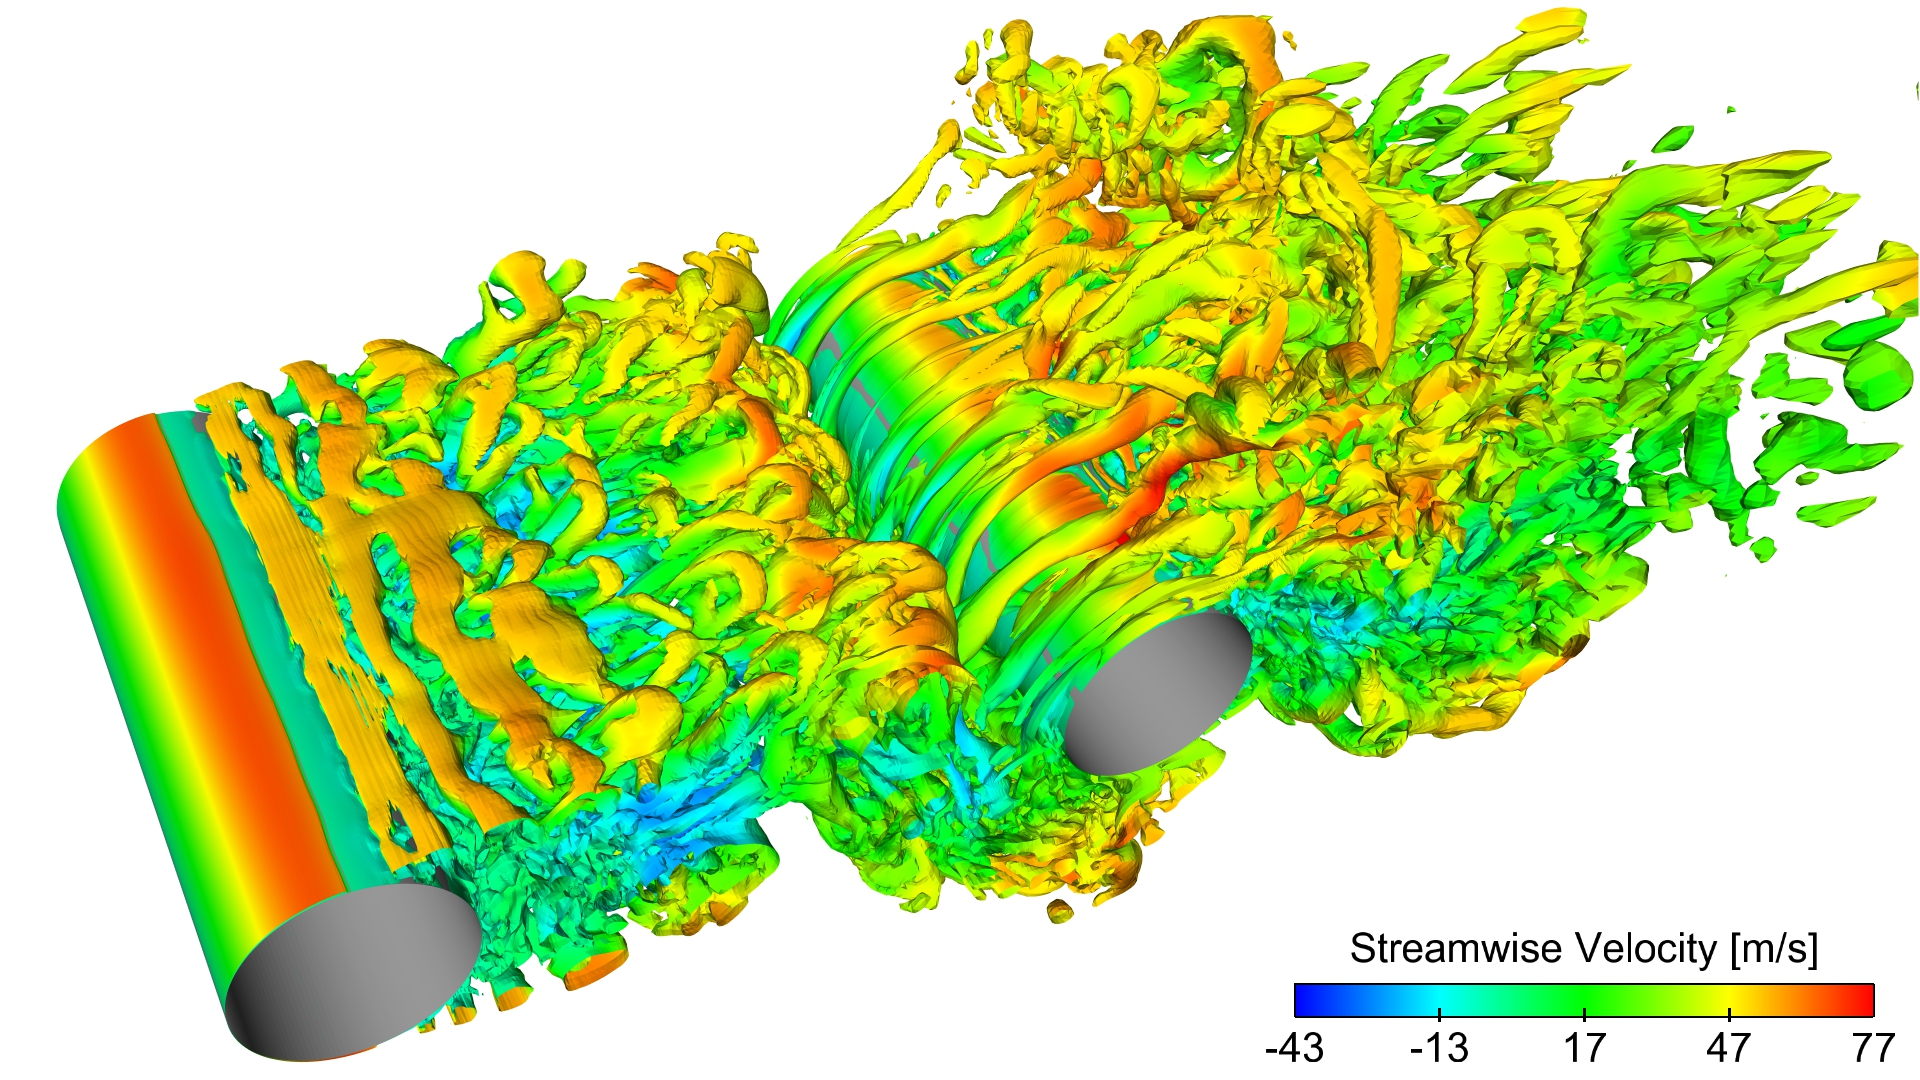
\includegraphics[width=0.45\textwidth]{tc_q_criteria}
    \caption{Q判据等值面图}
    \label{fig:tc_q_criteria}
\end{figure}
\end{verbatim}
\begin{figure}[!htbp]
    \centering
    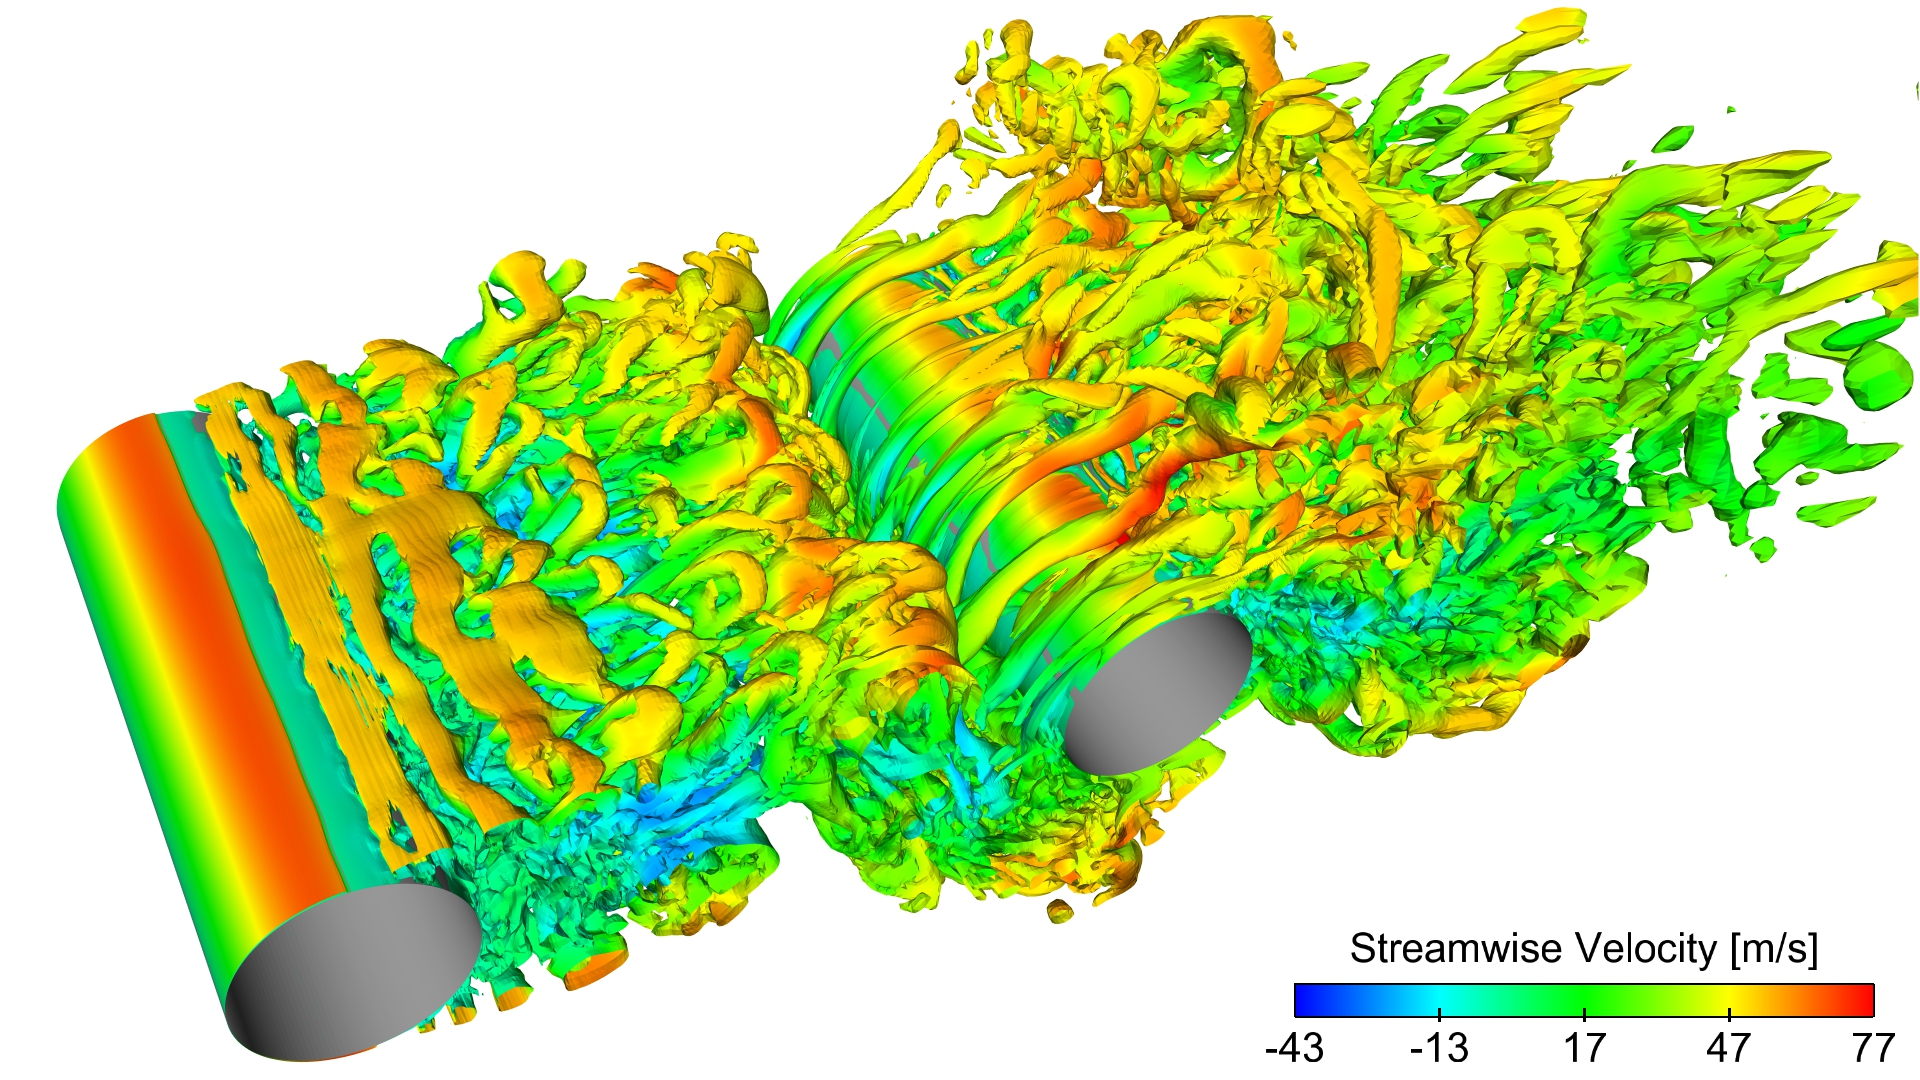
\includegraphics[width=0.45\textwidth]{tc_q_criteria}
    \caption{Q判据等值面图}
    \label{fig:tc_q_criteria}
\end{figure}

如果插图的空白区域过大,希望减少插入图片后的留白,以图片\verb|shock_cyn|为例(图\ref{fig:shock_cyn}),可以使用如下代码模板:
\begin{verbatim}
\begin{figure}[!htbp]
    \centering
    %trim option's parameter order: left bottom right top
    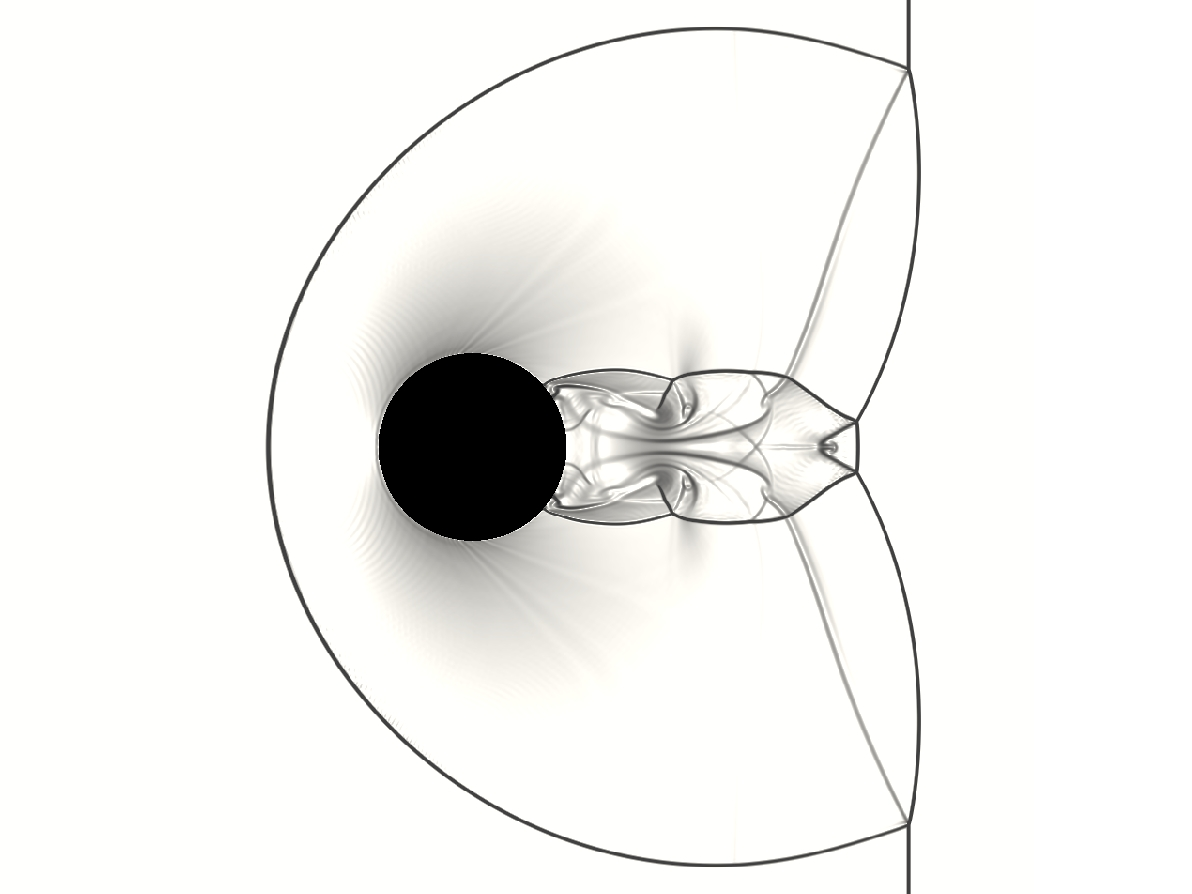
\includegraphics[trim = 30mm 0mm 30mm 0mm, clip,
    width=0.40\textwidth]{shock_cyn}
    \caption{Shock diffraction}
    \label{fig:shock_cyn}
\end{figure}
\end{verbatim}
\begin{figure}[!htbp]
    \centering
    %trim option's parameter order: left bottom right top
    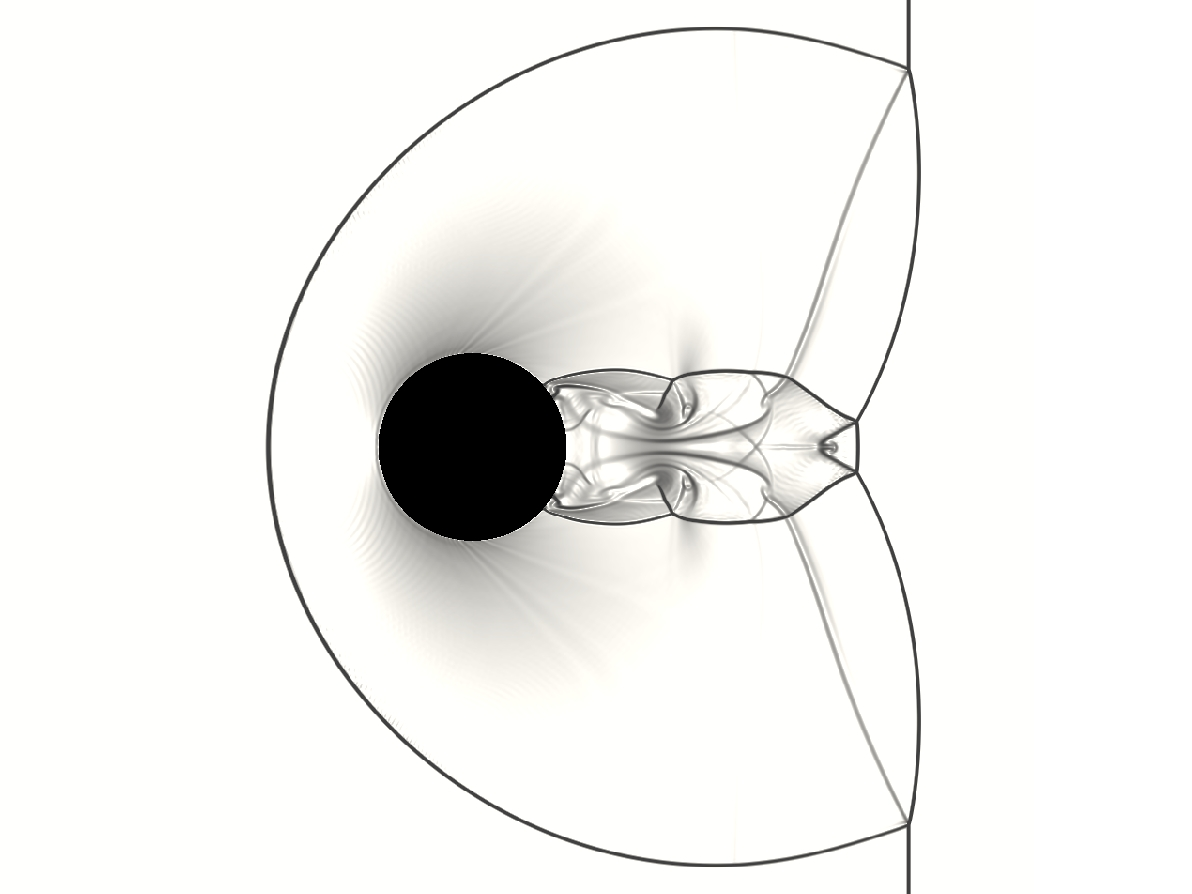
\includegraphics[trim = 30mm 0mm 30mm 0mm, clip, width=0.40\textwidth]{shock_cyn}
    \caption{激波圆柱作用。}
    \label{fig:shock_cyn}
\end{figure}

多图的插入如图\ref{fig:oaspl},其代码如下。
\begin{verbatim}
\begin{figure}[!htbp]
    \centering
    \begin{subfigure}[b]{0.45\textwidth}
      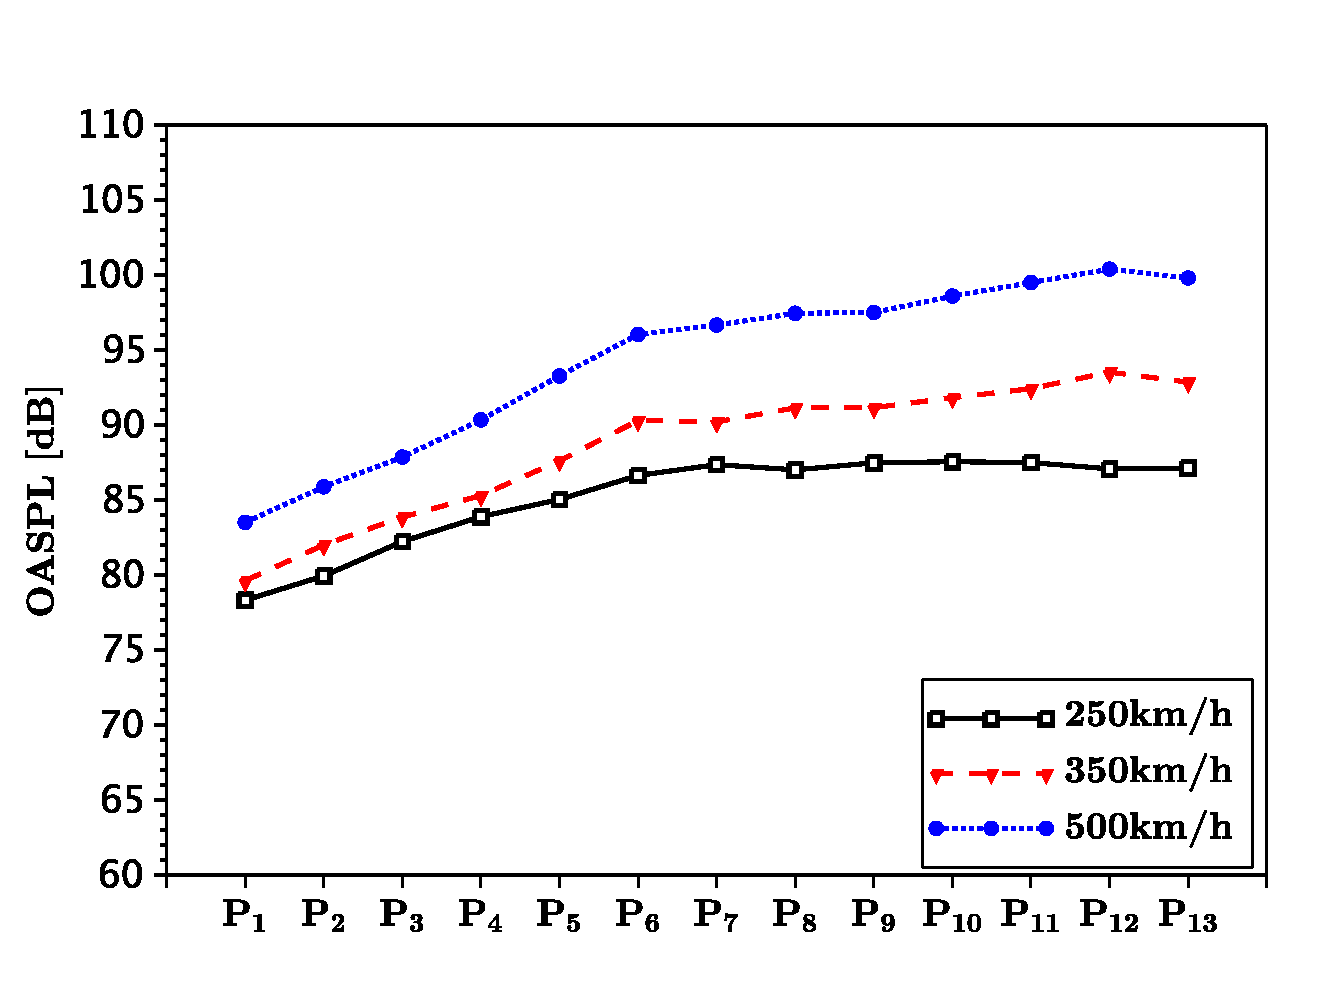
\includegraphics[width=\textwidth]{oaspl_a}
      \caption{}
      \label{fig:oaspl_a}
    \end{subfigure}%
    ~%add desired spacing
    \begin{subfigure}[b]{0.45\textwidth}
      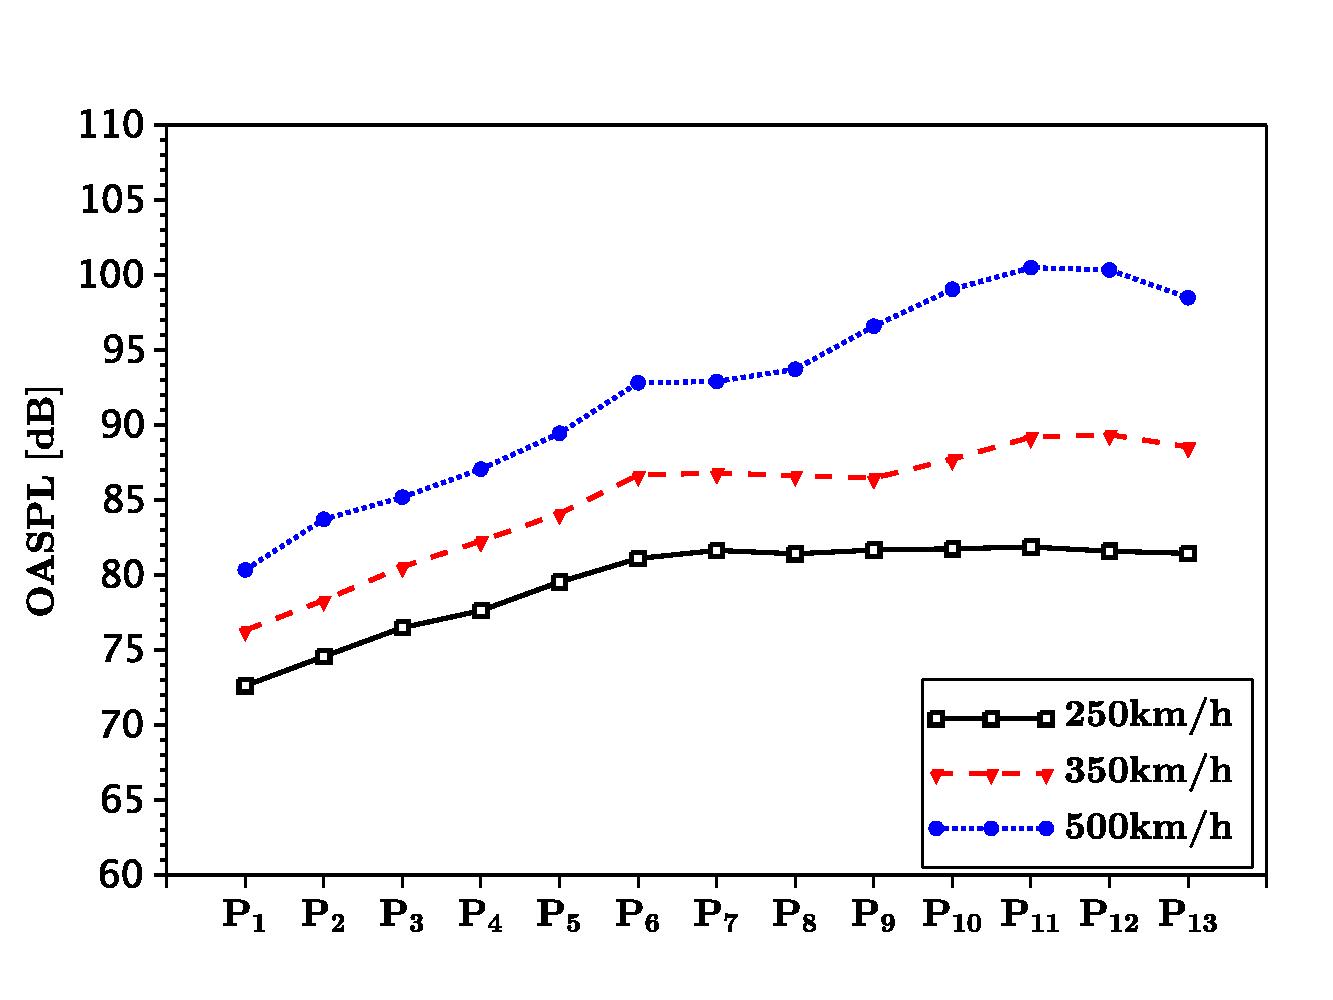
\includegraphics[width=\textwidth]{oaspl_b}
      \caption{}
      \label{fig:oaspl_b}
    \end{subfigure}
    \begin{subfigure}[b]{0.45\textwidth}
      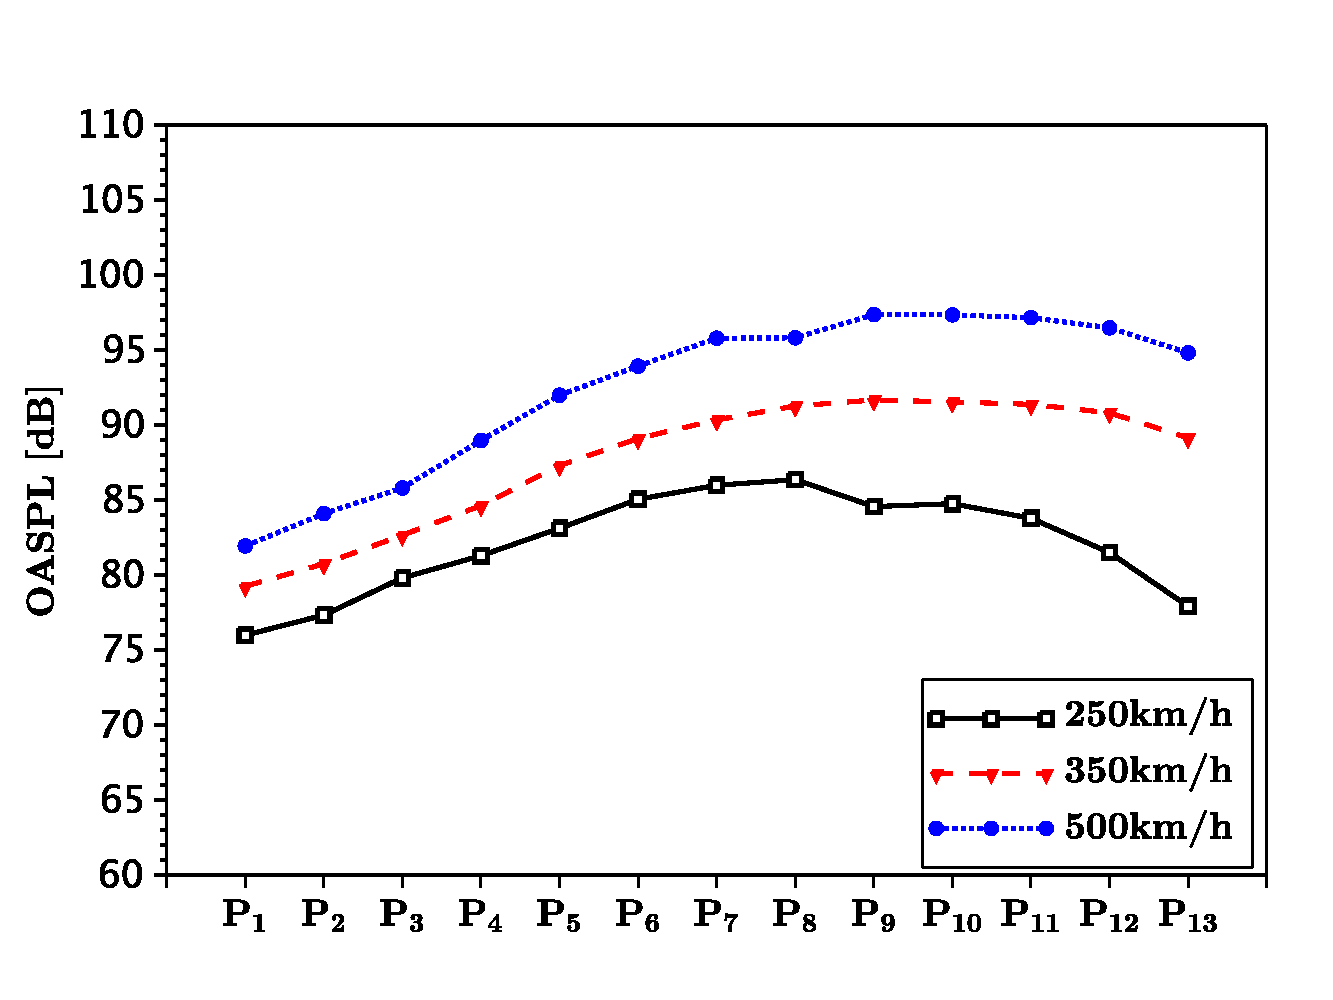
\includegraphics[width=\textwidth]{oaspl_c}
      \caption{}
      \label{fig:oaspl_c}
    \end{subfigure}%
    ~%add desired spacing
    \begin{subfigure}[b]{0.45\textwidth}
      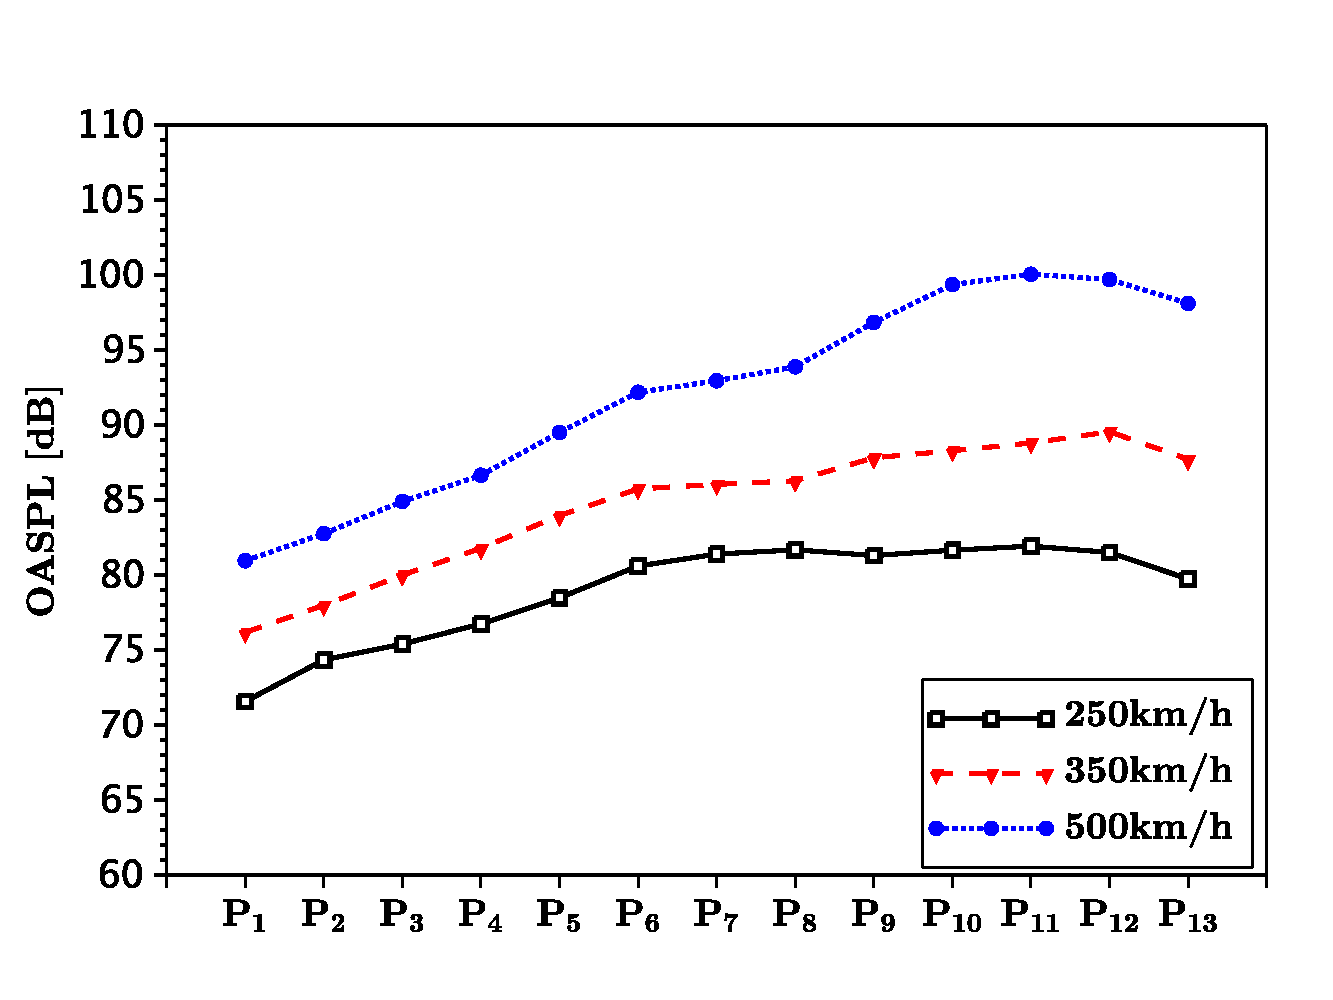
\includegraphics[width=\textwidth]{oaspl_d}
      \caption{}
      \label{fig:oaspl_d}
    \end{subfigure}
    \caption{总声压级。(a)$A$,(b)$B$,(c)$C$,(d)$D$}
    \label{fig:oaspl}
\end{figure}
\end{verbatim}
\begin{figure}[!htbp]
    \centering
    \begin{subfigure}[b]{0.45\textwidth}
      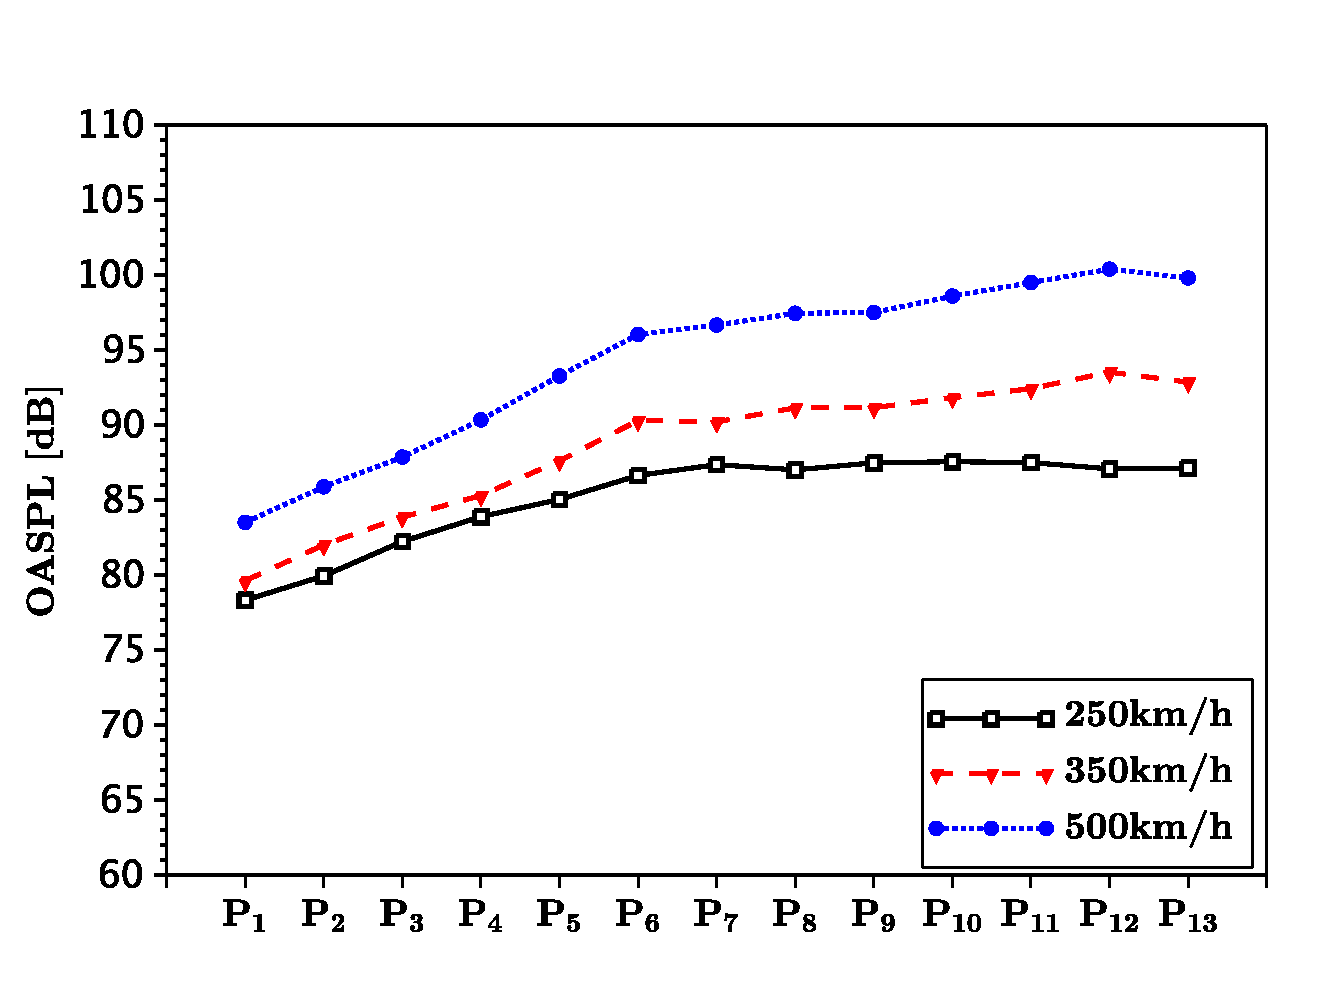
\includegraphics[width=\textwidth]{oaspl_a}
      \caption{}
      \label{fig:oaspl_a}
    \end{subfigure}%
    ~%add desired spacing
    \begin{subfigure}[b]{0.45\textwidth}
      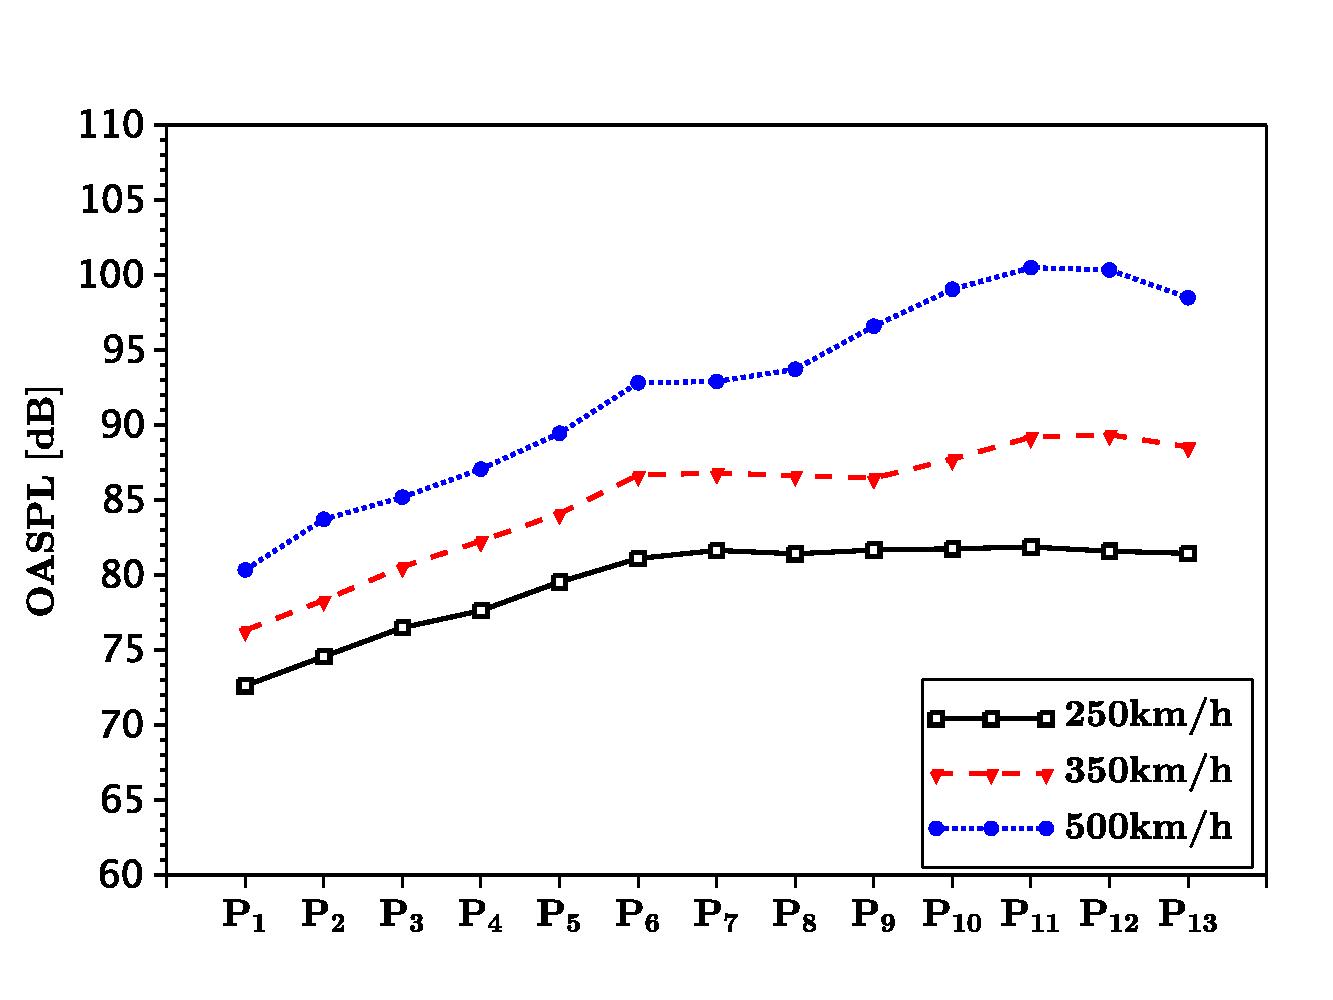
\includegraphics[width=\textwidth]{oaspl_b}
      \caption{}
      \label{fig:oaspl_b}
    \end{subfigure}
    \begin{subfigure}[b]{0.45\textwidth}
      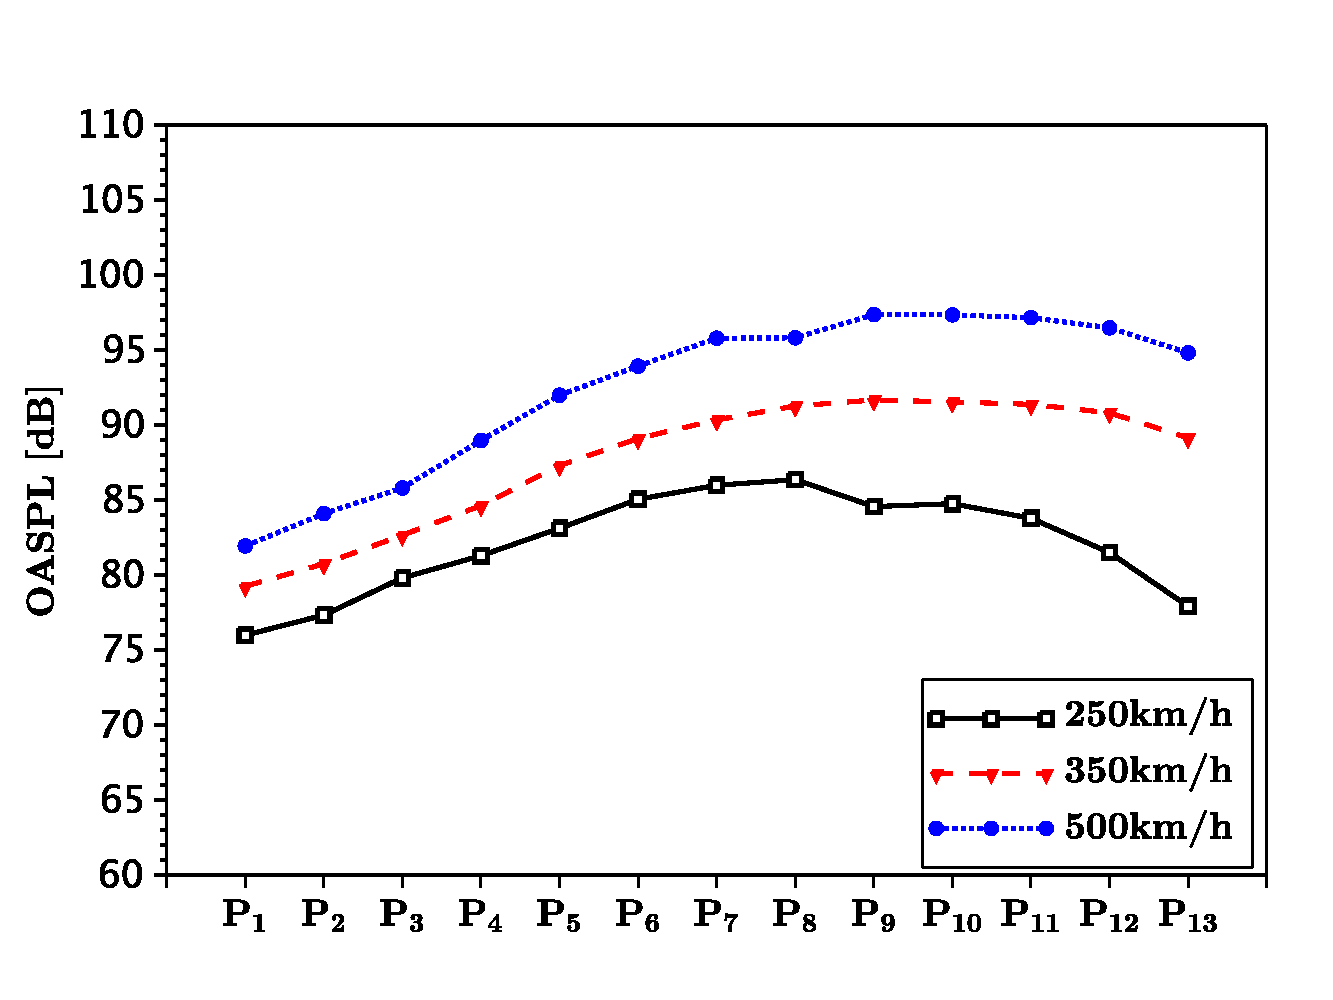
\includegraphics[width=\textwidth]{oaspl_c}
      \caption{}
      \label{fig:oaspl_c}
    \end{subfigure}%
    ~%add desired spacing
    \begin{subfigure}[b]{0.45\textwidth}
      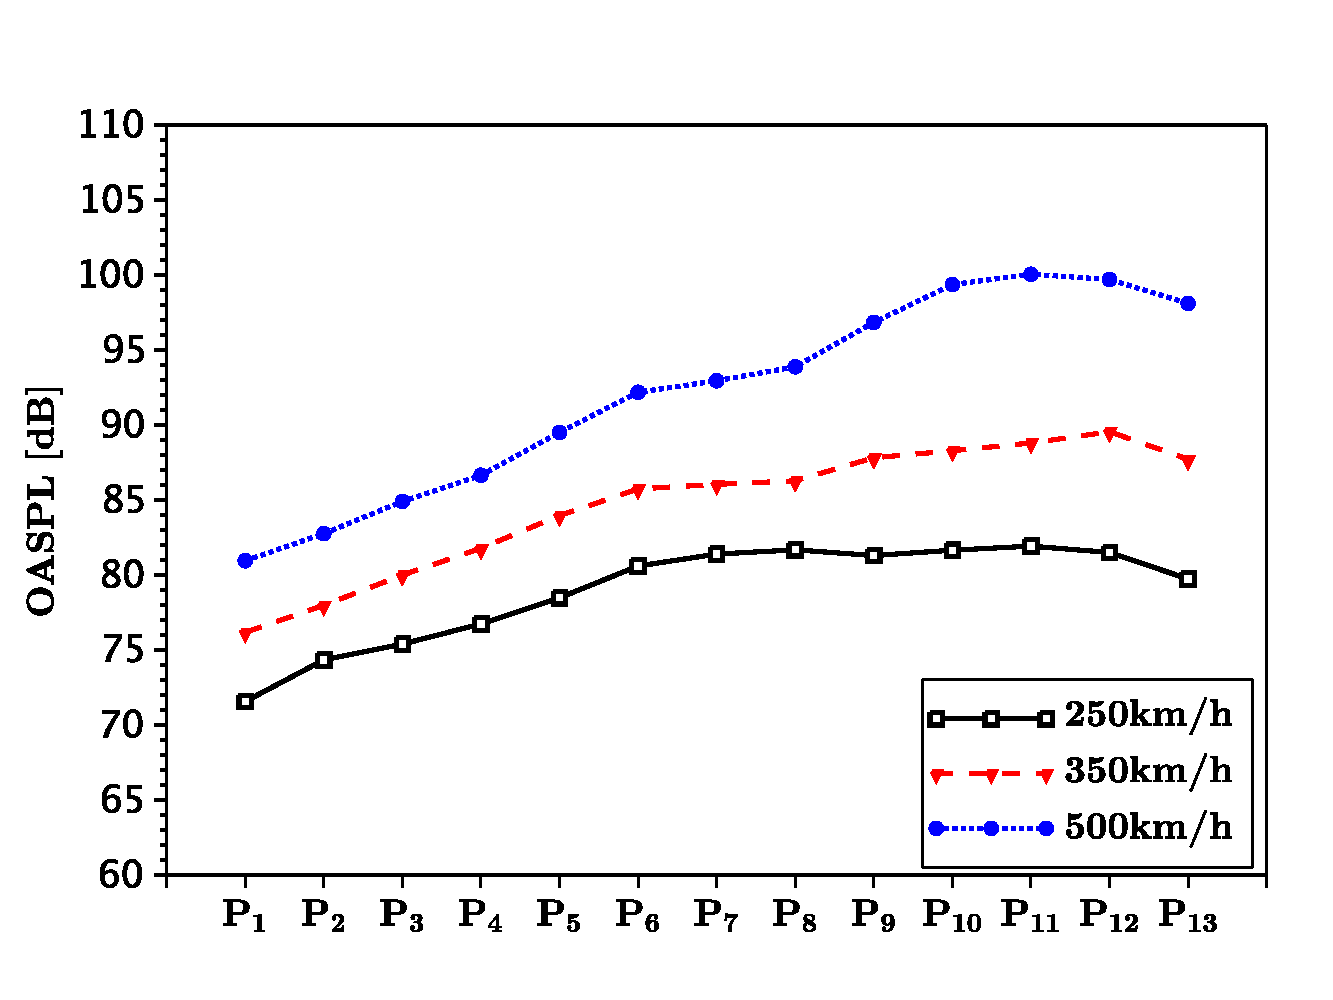
\includegraphics[width=\textwidth]{oaspl_d}
      \caption{}
      \label{fig:oaspl_d}
    \end{subfigure}
    \caption{总声压级。(a)$A$,(b)$B$,(c)$C$,(d)$D$}
    \label{fig:oaspl}
\end{figure}

撰写论文中,插图和制表常用到的命令,已在\verb|Tex/Commands.tex|这个文本中给出了参考代码,大家只需拷贝使用即可。

\subsection{参考文献引用}

参考文献引用过程以实例进行介绍,假设需要引用名为"Document Preparation System"的文献,步骤如下:

1)使用Google Scholar搜索Document Preparation System,在目标条目下点击Cite,展开后选择Import into BibTeX打开此文章的BibTeX索引信息,将它们copy添加到ref.bib文件中(此文件位于Biblio文件夹下)。

2)你会发现索引信息中第一行为 \verb|@article{lamport1986document,|。其中 \verb|lamport1986document| 即为此文献的label (\textbf{中文文献也必须使用英文label},一般遵照:姓氏拼音+年份+标题第一字拼音的格式),想要在论文中索引此文献,有两种索引类型:

文本类型:\verb|\citet{lamport1986document}|。正如此处所示 \citet{lamport1986document}; 

括号类型:\verb|\citep{lamport1986document}|。正如此处所示 \citep{lamport1986document}。

\textbf{多文献索引用英文逗号隔开}:

\verb|\citep{lamport1986document,chen2005zhulu}|。正如此处所示 \citep{lamport1986document,chen2005zhulu}

如此,即完成了文献的索引,请查看下本文档的参考文献一章,看看是不是就是这么简单呢?是的,就是这么简单!

不同文献样式和引用样式可在Thesis.tex中对artratex.sty调用实现,如:
\begin{itemize}
    \footnotesize
    \item \verb+\usepackage[numbers]{artratex}+ $\%$ 文本: Jones [1]; 括号: [1]
    \item \verb+\usepackage[super]{artratex}+ $\%$ 文本: Jones 上标[1]; 括号: 上标[1]
    \item \verb+\usepackage[authoryear]{artratex}+ $\%$ 文本: Jones (1995); 括号: (Jones, 1995)
    \item \verb+\usepackage[alpha]{artratex}+ $\%$ 文本: 不可用; 括号: [Jon95]
\end{itemize}

若在上标(super)模式下,希望在特定位置将上标改为嵌入式标,可使用

文本类型:\verb|\citetns{lamport1986document,chen2005zhulu}|。

正如此处所示\citetns{lamport1986document,chen2005zhulu}

括号类型:\verb|\citepns{lamport1986document,chen2005zhulu}|。

正如此处所示\citepns{lamport1986document,chen2005zhulu}

参考文献索引更为详细的信息,请见Wikibook\citep{wikibook2014latex} \nocite{*}。

\section{常见使用问题}\label{sec:qa}

\begin{enumerate}
    \item 下载模板后,用脚本编译出现错误,则i)请下载并更新模板。请更新\LaTeX{}编译器和包裹库,以确保模板与编译器的匹配。ii) 编译中若出现缺乏包裹或字体并提示是否自动下载,请选择自动下载,即可解决大部分初始编译时所遇到的问题。本模板在每次修改的发布前,都已在Windows,Linux,MacOS系统的最近两个发行版的Texlive上测试通过。

    \item 模板文档的编码为UTF-8编码。所有文件都必须采用UTF-8编码,否则编译后生成的文档将出现乱码文本。若出现文本编辑器无法打开文档或打开文档乱码的问题,请检查您使用的编辑器对UTF-8编码的支持。如果使用WinEdt作为文本编辑器(不推荐使用),应在其Options -> Preferences -> wrapping选项卡下将两种Wrapping Modes中的内容:TeX;HTML;ANSI;ASCII|DTX...修改为:TeX;\textbf{UTF-8|ACP;}HTML;ANSI;ASCII|DTX...同时,取消Options -> Preferences -> Unicode中的Enable ANSI Format...选项。

    \item 推荐选择xelatex编译引擎编译中文文档。编译脚本的默认设定为xelatex编译引擎。你也可以选择不使用脚本编译,如直接使用 \TeX{}文本编辑器编译。注:\TeX{}文本编辑器编译的默认设定为pdflatex编译引擎,若选择xelatex编译引擎,请进入下拉菜单选择xelatex。为正确生成引用链接,需要进行全编译,其步骤为:\verb|xelatex + bibtex + xelatex + xelatex|。
    \item Texmaker使用简介
        \begin{enumerate}
            \item 使用 Texmaker 打开文档 Thesis.tex。
            \item 菜单 Options -> Define Current Document As 'Master Document'
            \item 菜单 User -> User Commands -> Edit User Commands -> Input Menu Item as 'Auto Build' -> Click 'wizard' -> add: xelatex + bibtex + xelatex + xelatex + pdf viewer -> Click 'OK'
            \item 使用 Auto Build 编译带有未生成引用链接的源文件,可以仅使用 xelatex 编译带有已经正确生成引用链接的源文件。
            \item 编译完成,View PDF,在pdf中'ctrl+click'可链接到相对应的源文件。
        \end{enumerate}

    \item 若编译过程中出现无法找到某些package的错误,如无法找到xcolor.sty,mathtools.sty,ctexbook.sty,newtext.sty等,\TeX{}编译程序一般可以自动下载和安装相应的文件,否则,请进入\LaTeX{}软件的Package Manager (Admin)确认启用Repository--Synchronize状态。下次编译过程中\TeX{}编译程序一般将自动下载安装\LaTeX{}宏包库。
    \item 模版的设计可能地考虑了适应性。致谢等所有条目都是通过最为通用的

        \verb+\chapter{item name}+  and \verb+\section*{item name}+

        来显式实现的 (请观察Backmatter.tex),从而可以随意添加,放置,和修改,如同一般章节。对于图表目录名称则可在ucasthesis.cfg中进行修改。

    \item 设置文档样式: 在artratex.sty中搜索关键字定位相应命令,然后修改
        \begin{enumerate}
            \item 正文行距:修改 \verb|\linespread{1.3}|
            \item 参考文献行距:修改\verb|\setlength{\bibsep}{0.0ex}|
            \item 目录显示subsection:修改\verb|\setcounter{tocdepth}{2}|
            \item 页眉页脚的设定:frontmatterstyle,mainmatterstyle,和backmatterstyle分别用于定义前言,主要内容,和附录的页眉页脚样式。                关于页眉页脚各个命令的作用和意义请参见fancyhdr的用户文档 \url{https://www.ctan.org/pkg/fancyhdr?lang=en}。同时参见ctex宏包用户文档
                
                \url{http://ctan.mirror.rafal.ca/language/chinese/ctex/ctex.pdf}

            \item 设置图2.3为图2-3: 设置
                {
                    \footnotesize
\begin{verbatim}
\renewcommand{\theequation}{\arabic{chapter}-\arabic{equation}}
\renewcommand{\thefigure}{\arabic{chapter}-\arabic{figure}}
\renewcommand{\thetable}{\arabic{chapter}-\arabic{table}}
\end{verbatim}
                }
             \item 字体控制。如果对字体控制有较高需求,请选择xelatex编译引擎,并设置需要的字体。
                 
                 如启用Times New Roman 作为英文字体,设置:

                 \verb|\setmainfont{Times New Roman}|

                若拷贝PDF内容到Word时存在乱码,解决方式是安装adobe字体库,在百度云盘:

                {
                    \scriptsize
                    \url{http://pan.baidu.com/share/home?uk=3188136325&view=share#category/type=0}
                }
                 
                 下载如下四种中文字体文件:
                 \begin{enumerate}
                     \footnotesize
                     \item AdobeFangsongStd-Regular.otf (adobe 仿宋)
                     \item AdobeHeitiStd-Regular.otf(adobe 黑体)
                     \item AdobeKaitiStd-Regular.otf(adobe 楷体)
                     \item AdobeSongStd-Light.otf(adobe 宋体)
                 \end{enumerate}
                下载后,双击安装字体。然后在Thesis.tex中设置启用adobe的字体:

                \verb+\documentclass[doublesided,fontset=adobe]{Style/ucasthesis}%+

              若模版出现宋体无法加粗的情形,这是由于你的系统缺乏完备的中文字体或是ctex宏包没有调用到你的系统字体。Windows和Linux用户通过采用上述的adobe字体方案一般可解决问题。MacOS的用户则必须设置调用系统自带的中文字体,方法是在
                
                \verb|\RequirePackage{fontspec}|
                
                行下添加如下中文字体调用命令:
                {
                    \footnotesize
\begin{verbatim}
\setCJKmainfont[BoldFont=Heiti SC,ItalicFont=Kaiti SC]{Songti SC Light}%
\setCJKsansfont{Heiti SC}%
\setCJKfamilyfont{zhsong}{Songti SC Light}%
\setCJKfamilyfont{zhhei}{Heiti SC}%
\setCJKfamilyfont{zhkai}{Kaiti SC}%
\end{verbatim}
                }
                
                因为模版的设定考虑兼顾不同操作系统(Windows, Linux, Mac OS)并兼顾pdflatex和xelatex,为了模版的健壮性,上述字体设置和调用方案并未作为原始设定。
        \end{enumerate}

    \item  一般规范下,章应开始于奇数页。从而若前一章结束于奇数页,则一空白页将被插入以保证上述规则。如想修改以取消空白页,有如下方案:
     \begin{itemize}
         \item 在thesis.tex的documentclass中用singlesided替代doublesided。这使文档不区分奇偶页,因此章可以开始于任意页。此方案将移除所有空白页,包括封面处的。同时,页眉页脚的设定不再区分奇偶页。
         \item 可以在ucasthesis.cls文件中,将cleardoublepage命令的定义修改为:

             \verb|\def\cleardoublepage{\clearpage}|

             这一命令使产生空白页的机制失效。这一方案将移除所有的空白页,包括封面处的。但与方案一不同的是,页面页脚的设定可以区分奇偶页。
         \item 在thesis.tex的documentclass中添加openany选项(openany与doublesided和printcopy都可搭配)。这一命令使章可以开始于任意页。同时,将artratex.sty中和thesis.tex中的cleardoublepage改为clearpage。此方案将移除所有的用于调整章的起始位置的空白页,而不包括封面处的。同时,页面页脚的设定可以区分奇偶页。
     \end{itemize}
      无论哪种方案都要注意对页眉页脚的影响并做出合适的调整。推荐是采用默认设置,尽量避免将精力花在这些无关紧要的细节上。\LaTeX{}的特点是标准化,而其导致的问题则是任何脱离标准的修改都将花费相当精力。对于电子档的论文,在thesis.tex的documentclass中,若不想使用doublesided,则可使用singlesided来减少空白页。而对于打印版,启用printcopy选项以替换doublesided/singlesided选项,这样可使奇偶页的排版在打印装订后更美观。

  \item 部分所也许对论文格式有不同的设定,\LaTeX{}用户亦无需担心,仍可放心地使用当前模板进行论文撰写,因为\LaTeX{}的特征就在于内容与格式的分离。在使用此模板完成论文的撰写后,任何形式的格式调整都可独立于内容进行,并可只需通过修改模板样式文件中的少数命令轻松快速完成,并无风险。
\end{enumerate}


